\documentclass[12pt, a4paper]{extarticle}
\usepackage{GOST}
\usepackage{array}
\usepackage{verbatim}
\usepackage[detect-all]{siunitx}
\usepackage{amsmath}
\usepackage{amssymb}
\usepackage[utf8]{inputenc}
\usepackage{hyperref}
\usepackage{tempora}

\makeatletter
\renewcommand\@biblabel[1]{#1.}
\makeatother

\usepackage{listings}
\lstset{ 
	language=Prolog,
	basicstyle=\small, 
	numbers=left, 
	numberstyle=\tiny,
	stepnumber=1,
	numbersep=5pt,
	showspaces=false,            
	showstringspaces=false,      
	showtabs=false,             
	frame=single,            % рисовать рамку вокруг кода
	tabsize=4,      
	commentstyle=\color{green},
	keywordstyle=\color{blue}\textbf,
	numberstyle=\scriptsize\color{gray}, % the style that is used for the line-numbers
	rulecolor=\color{black},
	captionpos=t,
	breaklines=true,         % автоматически переносить строки 
	breakatwhitespace=false, % переносить строки по пробелу
	%escapeinside={\#*}{*)} 
}



\begin{document}
	
\begin{table}[ht]
	\centering
	\begin{tabular}{|c|p{400pt}|} 
		\hline
		\begin{tabular}[c]{@{}c@{}} 
\includegraphics[scale=1]{source/b_logo.jpg} \\\end{tabular} &
		\footnotesize\begin{tabular}[c]{@{}c@{}}\textbf{Министерство~науки~и~высшего~образования~Российской~Федерации}\\\textbf{Федеральное~государственное~бюджетное~образовательное~учреждение}\\\textbf{~высшего~образования}\\\textbf{«Московский~государственный~технический~университет}\\\textbf{имени~Н.Э.~Баумана}\\\textbf{(национальный~исследовательский~университет)»}\\\textbf{(МГТУ~им.~Н.Э.~Баумана)}\\\end{tabular}  \\
		\hline
	\end{tabular}
\end{table}
\noindent\rule{\textwidth}{4pt}
\noindent\rule[14pt]{\textwidth}{1pt}
\hfill 
\noindent
\makebox{ФАКУЛЬТЕТ~}%
\makebox[\textwidth][l]{\underline{~«Информатика и системы управления»~~~~~~~~~~~~~~~~~~~~~~~~~~~~~~~~~}}%
\\
\noindent
\makebox{КАФЕДРА~}%
\makebox[\textwidth][l]{\underline{~«Программное обеспечение ЭВМ и информационные технологии»~}}%
\\

\begin{center}
	\vspace{1.5cm}
	{\bf\huge Отчёт\par}
	{\bf\Large по лабораторной работе № 11\par}
	\vspace{0.7cm}
\end{center}


\noindent
\makebox{\large{\bf Название:}~~~}
\makebox[\textwidth][l]{\large\underline{~Среда Visual Prolog 5.2~}}\\

\noindent
\makebox{\large{\bf Дисциплина:}~~~}
\makebox[\textwidth][l]{\large\underline{~Функциональное и логическое программирование~}}\\

\vspace{1.5cm}
\noindent
\begin{tabular}{l c c c c c}
	Студент      & ~ИУ7-65Б~               & \hspace{2.5cm} & \hspace{2cm}                 & &  Д.В. Сусликов \\\cline{2-2}\cline{4-4} \cline{6-6} 
	\hspace{3cm} & {\footnotesize(Группа)} &                & {\footnotesize(Подпись, дата)} & & {\footnotesize(И.О. Фамилия)}
\end{tabular}

\noindent
\begin{tabular}{l c c c c}
	Преподаватель & \hspace{5cm}   & \hspace{2cm}                 & & ~~~~~~Н.Б. Толпинская~~~~~~\\\cline{3-3} \cline{5-5} 
	\hspace{3cm}  &                & {\footnotesize(Подпись, дата)} & & {\footnotesize(И.О. Фамилия)}
\end{tabular}

\vspace{0.6cm}
\begin{center}	
	\vfill
	\large \textit {Москва, 2021}
\end{center}

\thispagestyle {empty}
\pagebreak

\clearpage


\textbf{Цель работы} - познакомиться со средой Visual Prolog, познакомиться со структурой программы: способом запуска и формой вывода результата.

\textbf{Задачи работы:} изучить принципы работы в среде VisualProlog, возможность получения однократного и многократного результата, изучить базовые конструкции языка Prolog, структуру программы Prolog, форму ввода исходных данных и вывода результатов работы программы.

\textbf{Задание:} Запустить среду Visual Prolog 5.2. Настроить утилиту TestGoal. Запустить тестовую программу, проанализировать реакцию системы и множество ответов. Разработать свою программу - "Телефонный справочник". Протестировать работу программу.

\textbf{Задание 1}\par
Настройка TestGoal\par

\begin{figure}[h!]
	\centering{
\includegraphics[scale=1]{source/1.png}}
	\caption{Создание нового проекта}
\end{figure}

\begin{figure}[h!]
	\centering{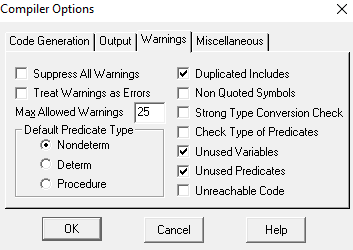
\includegraphics[scale=1]{source/2.png}}
	\caption{Настройка нового проекта}
\end{figure}

\newpage

\begin{figure}[h!]
	\centering{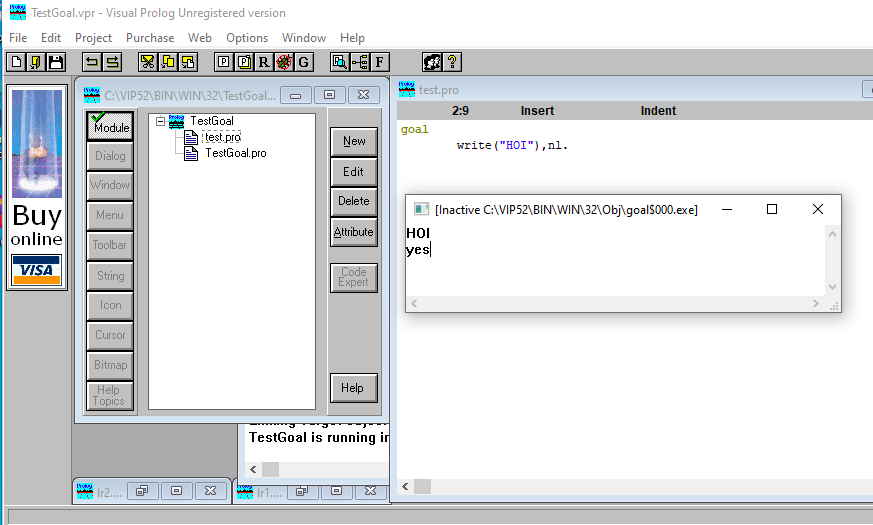
\includegraphics[scale=0.5]{source/3.png}}
	\caption{Запуск тестовой программы}
\end{figure}

\newpage
\textbf{Задание 2}\par
Разработать свою программу - "Телефонный справочник"\par

\begin{lstlisting}
predicates
	phonebook(symbol, symbol).
clauses
	phonebook("1111", "AAA").
	phonebook("2222", "BBB").
	phonebook("3333", "AAA").
	phonebook("444", "CCC").
goal
	phonebook(Number, "AAA").

\end{lstlisting}

Результат работы программы:
\begin{figure}[h!]
	\centering{
\includegraphics[scale=1]{source/4.png}}
	\caption{Результат}
\end{figure}

\newpage
\textbf{Ответы на вопросы:}
\begin{itemize}
	\item[1)] \textbf{Что собой представляет программа на Prolog?}
	Программа на Prolog представляет собой набор фактов и правил, которые
	формируют базу знаний о предметной области.
	Факты представляют собой составные термы, с помощью которых фиксируется
	наличие истинностных отношений между объектами предметной области —
	аргументами терма.
	Правила являются обобщенной формулировкой условия истинности знания –
	отношения между объектами предметной области (аргументами терма), которое
	записано в заголовке правила. Условие истинности этого отношения является
	телом правила.
	
	\item[2)] \textbf{Какова структура программы на Prolog?}\par
	Программа на Prolog состоит из разделов. Каждый раздел начинается со своего
	заголовка.\\
	Структура программы:\par
	\begin{itemize}
		\item директивы компилятора — зарезервированные символьные константы;
		\item CONSTANTS — раздел описания констант;
		\item DOMAINS — раздел описания доменов;
		\item DATABASE — раздел описания предикатов внутренней базы данных;
		\item PREDICATES — раздел описания предикатов;
		\item CLAUSES — раздел описания предложений базы знаний;
		\item GOAL — раздел описания внутренней цели (вопроса).
	\end{itemize}
	В программе не обязательно должны быть все разделы.
	
	\item[3)]  \textbf{Как реализуется программа на Prolog?}\par
	Описывается база знаний, задается вопрос.
	
	\item[4)] \textbf{Как формируются результаты работы программы?}\par
	В процессе выполнения программы — система пытается найти, используя базу
	знаний, такие значения переменных, при которых на поставленный вопрос
	можно дать ответ «Да».
\end{itemize}

\end{document}